\documentclass[12pt]{scrartcl}
\usepackage{minted}
\setminted{breaklines}
\usemintedstyle{tango}
\usepackage{booktabs}
\usepackage[polish]{babel}
\usepackage[dvipsnames]{xcolor}
\usepackage[colorlinks=true]{hyperref}
\hypersetup{urlcolor=MidnightBlue,linkcolor=DarkOrchid,citecolor=ForestGreen}
\usepackage{graphicx}
\usepackage{caption}
\usepackage{subcaption}
\newcommand{\sA}{\mathcal A}
\newcommand{\sB}{\mathcal B}
\newcommand{\sO}{\mathcal O}
\newcommand{\sS}{\mathcal S}

\title{Dokumentacja}
\author{Michał Dobranowski \and Wiktor Perczak}
\date{\today}


\begin{document}
\maketitle
\tableofcontents
\newpage

\section{Część techniczna}

\subsection{Wymagania}
Do używania programu potrzebny jest język \texttt{Python} w wersji co najmniej \texttt{3.10}. Ponadto wykorzystywane są również moduły:
\begin{itemize}
    \item \texttt{numpy 1.26.2}
    \item \texttt {bitalg} napisany przez koło naukowe BIT do wizualizacji danych: \url{https://github.com/aghbit/Algorytmy-Geometryczne}
\end{itemize}

\subsection{Moduł \texttt{geometry}}

\subsubsection{\texttt{Rectangle}}
Klasa Rectangle implementuje prostokąt oraz wiele operacji, które można na nim wykonać:
\begin{itemize}
    \item \texttt{def \_\_eq\_\_(self, other: Rectangle) -> bool} -- metoda sprawdzająca, czy dwa prostokąty są sobie równe (czy współrzędne ich wierzchołków są identyczne)
    \item \texttt{def \_\_and\_\_(self, other: Rectangle) -> Rectangle | None} -- metoda zwracająca część wspólną dwóch prostokątów, lub \texttt{None}, jeśli ona nie istnieje
    \item \texttt{def \_\_contains\_\_(self, item: Rectangle | Point) -> bool} -- metoda sprawdzająca, czy jeden prostokąt w pełni zawiera się w drugim
\end{itemize}

\subsection{Moduł \texttt{tree}}
Zawiera klasę abstrakcyjną \texttt{Tree}, po której dziedziczą \texttt{Quadtree} oraz \texttt{KdTree}. Posiada dwie metody:
\begin{itemize}
    \item \texttt{def \_\_init\_\_(self, points: list[Point])} -- konstruktor klasy
    \item \texttt{def find(self, rectangle: Rectangle) -> list[Point]} -- zwraca listę punktów, które znajdują się w zadanym prostokącie
\end{itemize}

\subsection{Moduł \texttt{quadtree}}
\subsubsection{\texttt{\_Node}}
Każdy obiekt \texttt{\_Node} trzyma informację o:
\begin{itemize}
    \item \texttt{self.rectangle} -- prostokącie, za który odpowiada dany wierzchołek drzewa
    \item \texttt{self.min\_x, self.max\_x, self.min\_y, self.max\_y} -- ekstremach prostokąta
    \item \texttt{self.mid\_x, self.min\_y} -- wartości w środku prostokąta
    \item \texttt{self.children} -- dzieciach danego wierzchołka
    \item \texttt{self.leaf\_node} -- współrzędnych punktu, jeśli wierzchołek jest liściem
\end{itemize}

\subsubsection{\texttt{Quadtree}}
Klasa \texttt{Quadtree} umożliwia budowanie drzewa czwórkowego oraz odpowiadanie na zapytania o punkty wewnątrz danego prostokąta. Posiada następujące metody:
\begin{itemize}
    \item \texttt{def \_\_init\_\_(self, points: list[Point])} -- tworzy pierwszy (największy) prostokąt, który zostaje zapisany w korzeniu drzewa (\texttt{self.root}). Nastepnie wywołuje z korzenia metodę \texttt{\_\_construct\_subtree}, która konstruuje drzewo czwórkowe.
    \item \texttt{ \_\_construct\_subtree(self, node: \_Node, points: list[Point])} -- konstruuje drzewo czwórkowe, dzieląc kolejne prostokąty na cztery ćwiartki oraz rozdzielając odpowiednio punkty na cztery zbiory. Jeżeli dojdzie do prostokąta, wewnątrz którego jest tylko jeden punkt, to obecnie rozważany wierzchołek (\texttt{\_Node}) staje się liściem drzewa.

    Złożoność: $\sO(hn)$, gdzie $h$ to wysokość drzewa czwórkowego.
    \item  \texttt{def \_\_find(self, node: \_Node, rectangle: Rectangle, res: list[Point])} -- metoda, która służy do znajdywania punktów wewnątrz zadanego prostokąta. Rekurencyjnie znajduje prostokąty, które w pełni zawierają się w prostokącie z zapytania i dodaje liście poniżej do odpowiedzi.
    \item \texttt{def find(self, rectangle: Rectangle) -> list[Point]} -- wywołuje metodę \texttt{\_\_find()} i zwraca listę punktów, które mieszczą się w zadanym prostokącie. Złożoność: $\sO(hk)$, gdzie $k$ to liczba znalezionych punktów.
\end{itemize}

\subsection{Moduł \texttt{kd\_tree}}

\subsubsection{\texttt{\_Node}}
Każdy obiekt \texttt{\_Node} trzyma informację o:
\begin{itemize}
    \item \texttt{self.left} -- lewym dziecku wierzchołka
    \item \texttt{self.right} -- prawym dziecku wierzchołka
    \item \texttt{self.rectangle} -- prostokącie, który powstał przez ograniczenia przodków
    \item \texttt{self.leafs} -- liście wszystkich liści, które są potomkami danego wierzchołka
    \item \texttt{self.leaf\_point} -- współrzędnych punktu, jeśli dany wierzchołek jest liściem
\end{itemize}

\subsubsection{\texttt{KdTree}}
Klasa \texttt{KdTree} umożliwia budowanie drzewa oraz odpowiadanie na zapytania 2D, gdyż taki był temat zadania. Kod można jednak bardzo łatwo przekształcić, tak aby umożliwiał operacje na dowolnej liczbie wymiarów. Klasa \texttt{KdTree} posiada następujące metody:
\begin{itemize}
    \item \texttt{def \_\_init\_\_(self, points: list[Point])} -- konstruktor klasy, do którego przekazuje się listę punktów, a następnie konstruowane jest kd-drzewo. Tworzony jest też parametr \texttt{self.root}, dzięki któremu ma się dostęp do całego drzewa.
    \item \texttt{def build\_tree(self, points: list[Point], depth: int, rectangle: Rectangle) -> \_Node} -- metoda, która rekurencyjnie buduje kd-drzewo. W każdej instancji dzieli dany zbiór punktów na dwa zbiory względem współrzędnej podziału, którą jest mediana (wyliczana algorytmem \texttt{quick\_select}). Następnie wywołuje się rekurencyjnie z dzieci wierzchołka, który jest obecnie rozważany. W liściach zapisuje punkty z zadanego zbioru.
    Złożoność: $\sO(n \log n)$.
    \item \texttt{def \_\_find(self, node: \_Node, rectangle: Rectangle, res: list[Point])} -- metoda, która służy do znajdywania punktów wewnątrz zadanego prostokąta. Jeśli prostokąt z danego wierzchołka w pełni zawiera się, w prostokącie z zapytania to dodaje do odpowiedzi wszystkie liście poniżej. Jeśli zawiera się tylko częściowo, wywołuje się rekurencyjnie z jego dzieci.
    \item \texttt{def find(self, rectangle: Rectangle) -> list[Point]} -- wywołuje metodę \texttt{\_\_find()} i zwraca listę punktów, które mieszczą się w zadanym prostokącie.
    Złożoność: $\sO(\sqrt n + k)$, gdzie $k$ to liczba znalezionych punktów.
\end{itemize}

\subsection{Moduł \texttt{quick\_select}}
Służy do zwracania mediany nieposortowanego zbioru punktów w czasie $\sO(n)$. Działanie jest identyczne z sortowaniem przez scalanie, dzieli zbiór na dwa zbiory względem zadanej wartości, aż odnajdzie medianę. Posiada trzy funkcje:
\begin{itemize}
    \item \texttt{def quick\_select(points: list[Point], l: int, r: int, k: int, depth: int) -> Point} -- zwraca medianę zbioru punktów, względem danego wymiaru (\texttt{depth: int})
    \item \texttt{def partition(points: list[Point], l: int, r: int, depth: int) -> int} -- porządkuje punkty na dwa zbiory: mniejsze od punktu porządkującego lub większe od niego i zwraca indeks pierwszego punktu ze zbioru punktów większych od punktu porządkującego
    \item \texttt{def rand\_partition(points: list[Point], l: int, r: int, depth: int) -> int} -- losowo wybiera punkt porządkujący, a następnie wywołuje funkcję \texttt{partition()}
\end{itemize}

\section{Część użytkownika}
W tej sekcji zaprezentowane są przykładowe użycia klas \texttt{Quadtree} i \texttt{KdTree}: skonstruowanie drzewa oraz znalezienie punktów, leżących wewnątrz zadanego prostokąta.

\subsection{Użycie Quadtree}
\begin{minted}{python}
from quadtree import Quadtree
from geometry import Rectangle

points = [(0, 0), (1.5, 1), (2, 3), (2, 0), (0.5, 1.5)]
rectangle = Rectangle(0, 1.5, 1, 3)

tree = Quadtree(points)
print(tree.find(rectangle))
\end{minted}

Odpowiedź dla przykładu: [(0.5, 1.5), (1.5, 1)].

\subsection{Użycie KdTree}
\begin{minted}{python}
from kd_tree import KdTree
from geometry import Rectangle

points = [(0, 0), (1.5, 1), (2, 3), (2, 0), (0.5, 1.5)]
rectangle = Rectangle(0, 1.5, 1, 3)

tree = KdTree(points)
print(tree.find(rectangle))
\end{minted}

\section{Wizualizacja}
Do wizualizacji wykorzystano narzędzie koła naukowego BIT (\url{https://github.com/aghbit/Algorytmy-Geometryczne}). Napisano dwie klasy \texttt{QuadtreeVis} oraz \texttt{KdTreeVis}, które umożliwiają:
\begin{itemize}
    \item podział przestrzeni na prostokąty
    \item zobrazowanie zbioru znalezionych punktów dla danego zapytania
    \item wygenerowanie pliku GIF, który wizualizuje kolejne kroki algorytmu
\end{itemize}

\subsection{Wizualizacja \texttt{QuadtreeVis}}
Klasa \texttt{QuadtreeVis} dziedziczy po \texttt{Quadtree} dodatkowo dodając elementy wizualizacji.

Przykładowy kod na zwizualizowanie procesu tworzenia quadtree (na losowo wygenerowanym zbiorze):

\begin{minted}{python}
from quadtree_visualization import QuadtreeVis
from geometry import Rectangle
from numpy.random import seed, uniform

def generate_uniform_points(left, right, n):
    return list(zip(uniform(left, right, size=n), uniform(left, right, size=n)))

points = generate_uniform_points(-10, 10, 25)
rectangle = Rectangle(-3, 1, -7, 5)
quadtree = QuadtreeVis(points)
quadtree.add_grid()
quadtree.find(rectangle)
quadtree.vis.show()
\end{minted}

Wykres wygenerowany przez ten program przedstawia poniższy rysunek.

\begin{figure}[H]
    \centering
    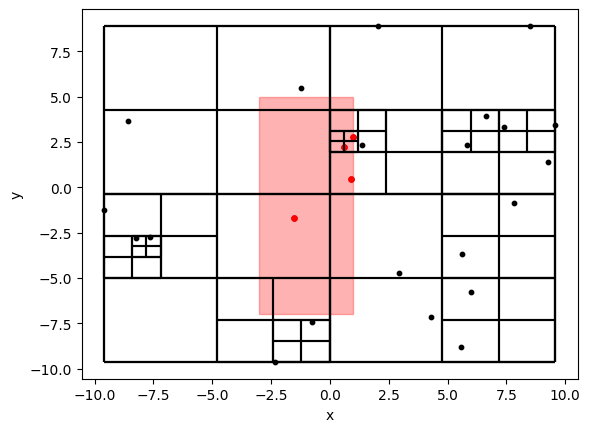
\includegraphics[width=0.7\textwidth]{imgs/quadtree_vis.png}
    \caption{Wizualizacja drzewa czwórkowego.}
\end{figure}

Aby wygenerować plik GIF do wyświetlania kolejnych kroków algorytmu, należy zamiast: \texttt{quadtree.vis.show()}, użyć \texttt{quadtree.vis.show\_gif()}.

\subsection{Wizualizacja \texttt{KdTreeVis}}
Klasa \texttt{KdTreeVis} działa identycznie jak klasa \texttt{KdTree}, ale dodatkowo dodaje elementy wizualizacji, zarówno podczas konstruowania drzewa, jak i odpowiadania na zapytanie.

Przykładowe użycie klasy \texttt{KdTreeVis} dla losowo wygenerowanego zbioru punktów:

\begin{minted}{python}
from kd_tree_visualization import KdTreeVis
from geometry import Rectangle
from numpy.random import seed, uniform

def generate_uniform_points(left, right, n):
    return list(zip(uniform(left, right, size=n), uniform(left, right, size=n)))

points = generate_uniform_points(-10, 10, 25)
rectangle = Rectangle(-3, 1, -7, 5)
kd_tree = KdTreeVis(points)
kd_tree.find(rectangle)
kd_tree.vis.show()
\end{minted}

Wykres wygenerowany przez ten program przedstawia poniższy rysunek.

\begin{figure}[H]
    \centering
    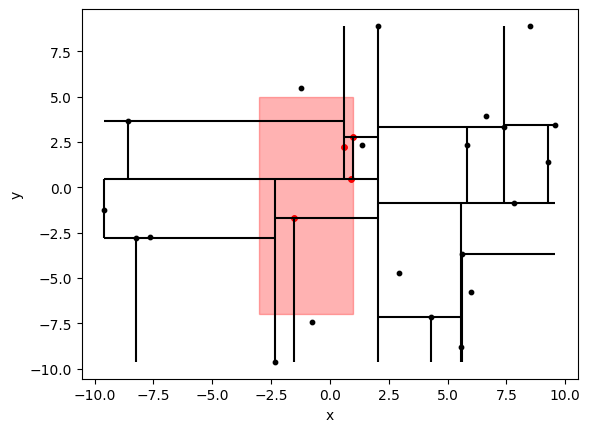
\includegraphics[width=0.7\textwidth]{imgs/kd_tree_vis}
    \caption{Wizualizacja kd-drzewa.}
\end{figure}

Aby wygenerować plik GIF do wyświetlania kolejnych kroków algorytmu, należy zamiast:
\texttt{kd\_tree.vis.show()}, użyć \texttt{kd\_tree.vis.show\_gif()}.

\section{Porównanie -- testy czasowe}
Porównanie obu struktur danych przeprowadzono przy użyciu dwóch zbiorów testujących:
\begin{itemize}
    \item $\sA(n)$ -- zbiór $n$ punktów $P \in \sS = [-1000, 1000]^2$ wygenerowanych losowo za pomocą funkcji \texttt{numpy.random.uniform},
    \item $\sB(n)$ -- zbiór $n$ punktów, z których połowa to zbiór $\sA(n/2)$, a reszta to translacja tego zbioru o wektor $[10^{-8}, 0]$.
\end{itemize}

Dla każdego zbioru wybrano po $5$ wartości $n$, dla których przeprowadzono testy. Każdy z testów polegał na wygenerowaniu $15$ zbiorów testujących i sprawdzenia czasu wykonywania:
\begin{enumerate}
    \item konstrukcji drzewa,
    \item zapytania o mały prostokąt (losowy, mający powierzchnię równą $\frac{1}{100}$ powierzchni prostokąta $\sS$),
    \item zapytania o duży prostokąt (losowy, mający powierzchnię równą $\frac{1}{4}$ powierzchni prostokąta $\sS$),
\end{enumerate}
dla każdej ze struktur. Średni czas dla każdej konfiguracji przedstawiono w tabelach \ref{tab:porównanie czasów A} i \ref{tab:porównanie czasów B} na końcu dokumentu.

\subsection{Wyniki}

Dla zbiorów typu $\sA$ drzewo czwórkowe okazało się wyraźnie lepsze. Szybciej można je skonstruować (rysunek \ref{fig:uniform construction time}), minimalnie szybciej również odpowiada na zapytania o duży prostokąt (rysunek \ref{fig:uniform find big time}). W zdecydowanie lepszym czasie odpowiada też na zapytania o mały prostokąt (rysunek \ref{fig:uniform find small time}).

\begin{figure}[H]
    \centering
    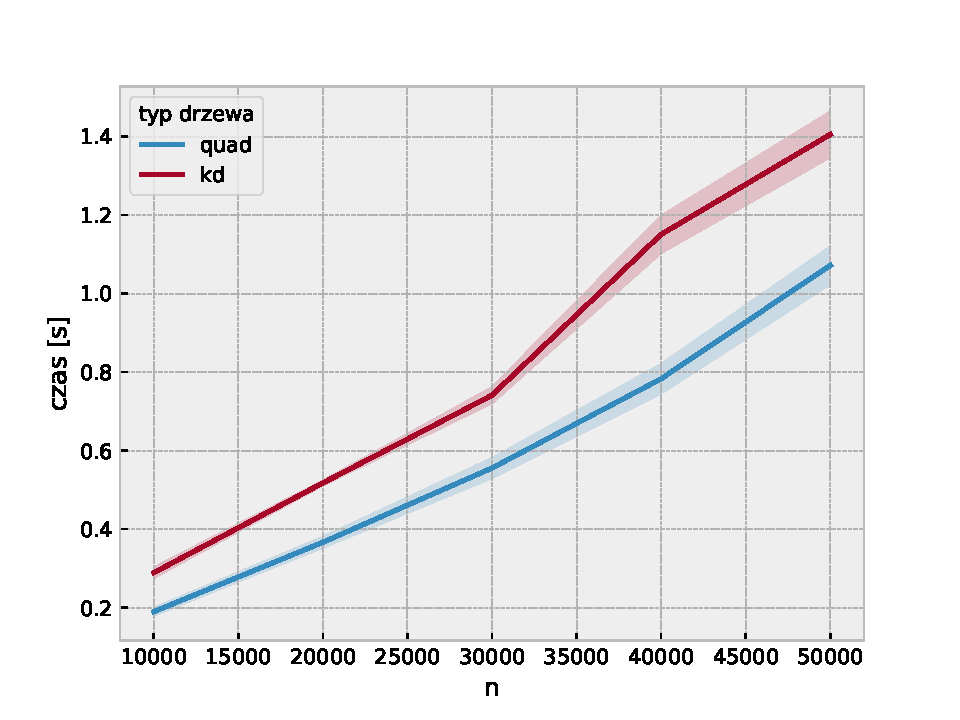
\includegraphics[width=0.65\textwidth]{imgs/uniform_construction_time}
    \caption{Porównanie czasu konstrukcji drzew dla zbioru $\sA$.}
    \label{fig:uniform construction time}
\end{figure}

\begin{figure}[H]
    \begin{subfigure}{0.5\textwidth}
        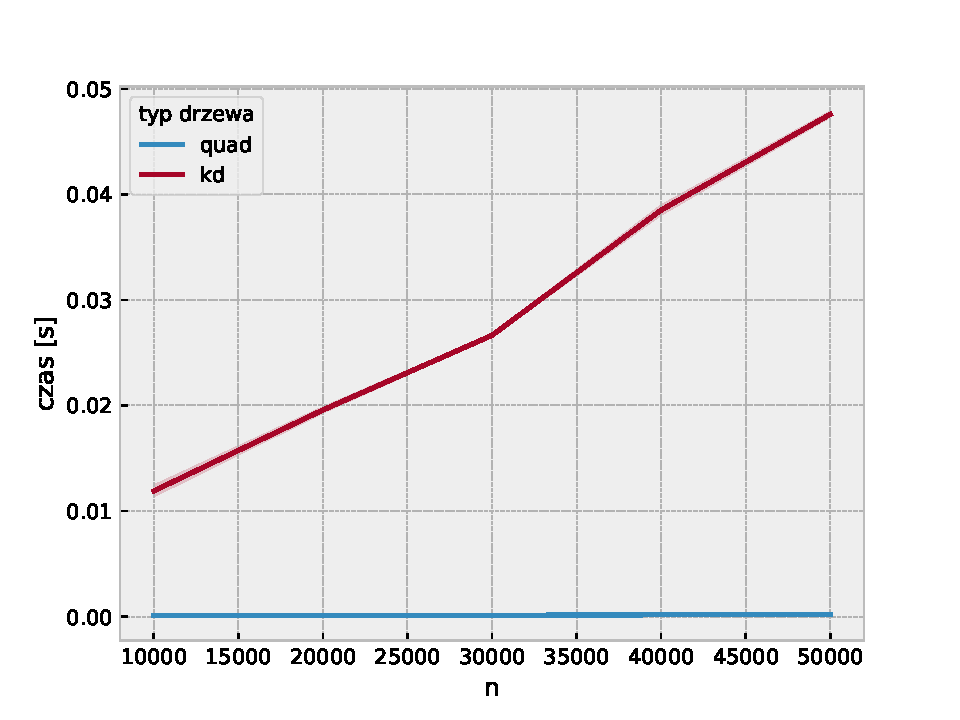
\includegraphics[width=\textwidth]{imgs/uniform_find_small_time}
        \caption{zapytania o mały prostokąt}
        \label{fig:uniform find small time}
    \end{subfigure}
    \begin{subfigure}{0.5\textwidth}
        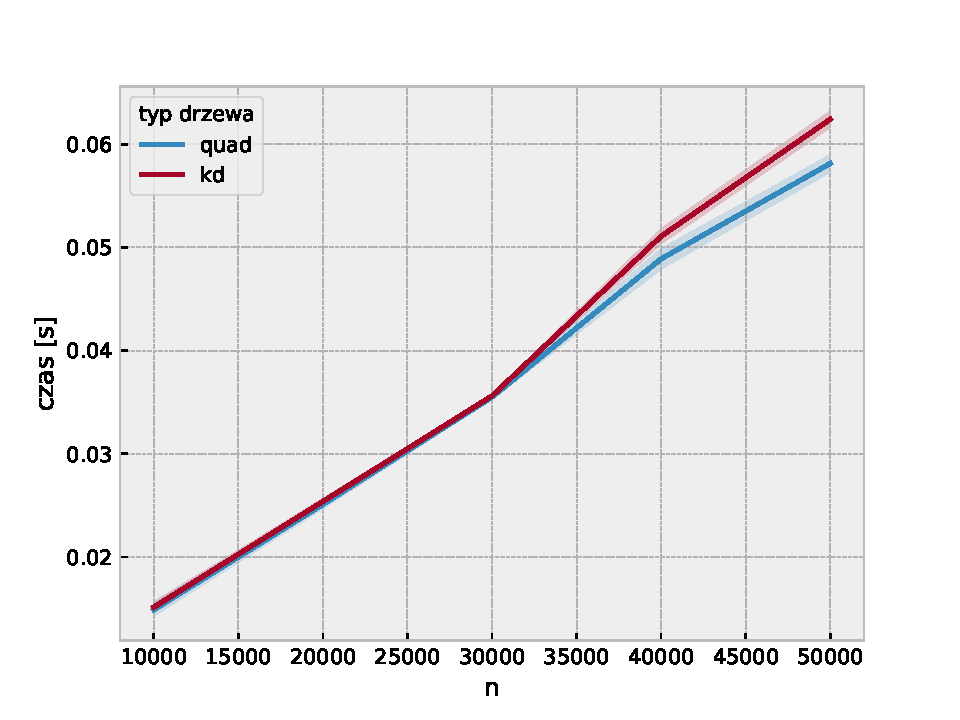
\includegraphics[width=\textwidth]{imgs/uniform_find_big_time}
        \caption{zapytania o duży prostokąt}
        \label{fig:uniform find big time}
    \end{subfigure}
    \caption{Porównanie czasu zapytania dla zbioru $\sA$.}
\end{figure}

Zupełnie inaczej wygląda sytuacja w przypadku zbiorów typu $\sB$. Zarówno konstrukcja drzewa czwórkowego, jak i użycie go dla zapytań o duży prostokąt, jest zdecydowanie wolniejsze niż w przypadku kd-drzewa (rysunki \ref{fig:pairs construction time} i \ref{fig:pairs find big time}). Różnica jest na tyle duża, że testy przeprowadzono na danych o rząd wielkości mniejszych. W zapytaniach o mały prostokąt ponownie lepiej sprawdza się drzewo czwórkowe (rysunek \ref{fig:pairs find small time}).

\begin{figure}[H]
    \centering
    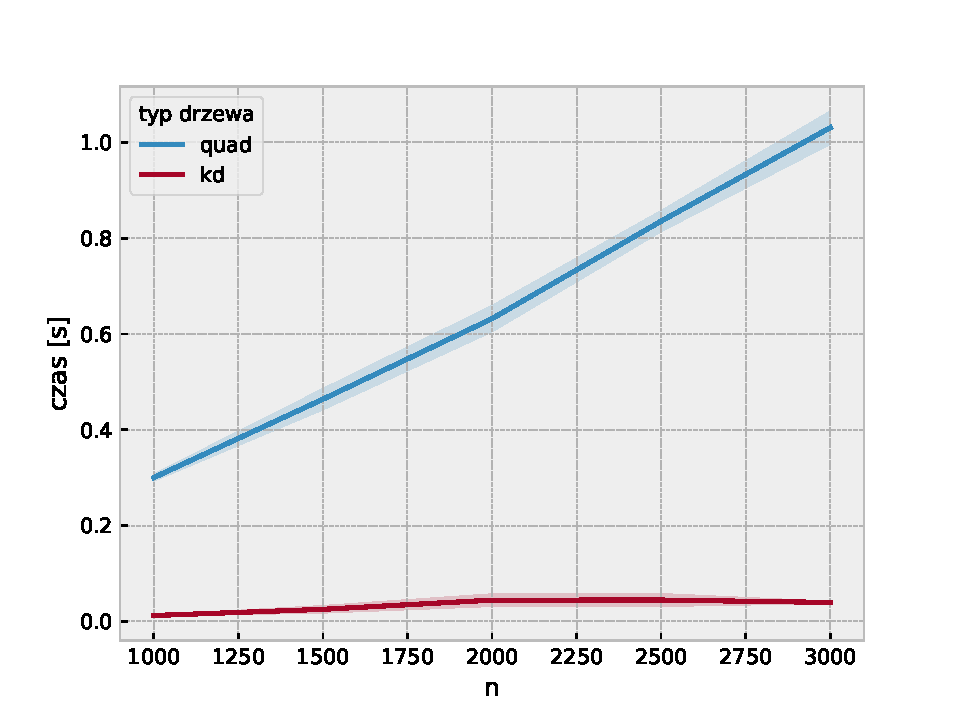
\includegraphics[width=0.65\textwidth]{imgs/pairs_construction_time}
    \caption{Porównanie czasu konstrukcji drzew dla zbioru $\sB$.}
    \label{fig:pairs construction time}
\end{figure}

\begin{figure}[H]
    \begin{subfigure}{0.5\textwidth}
        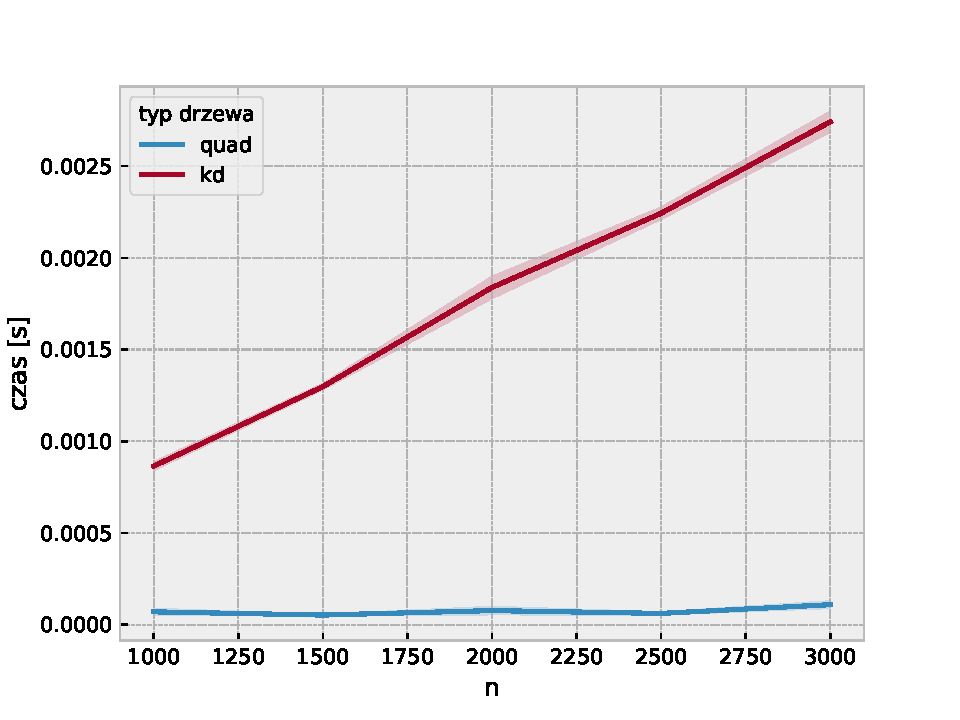
\includegraphics[width=\textwidth]{imgs/pairs_find_small_time}
        \caption{zapytania o mały prostokąt}
        \label{fig:pairs find small time}
    \end{subfigure}
    \begin{subfigure}{0.5\textwidth}
        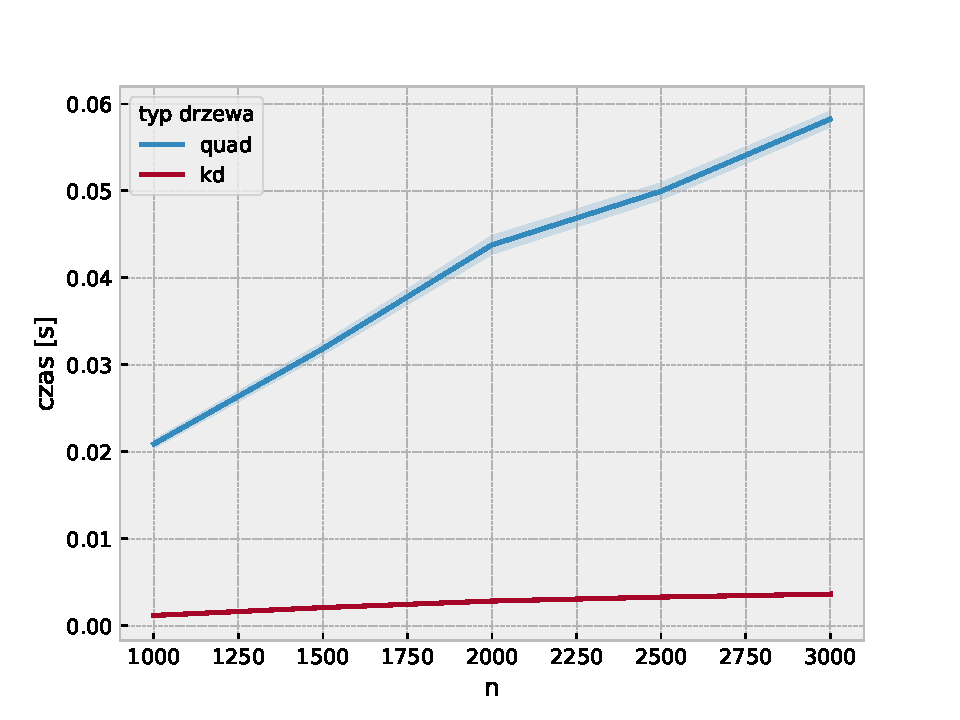
\includegraphics[width=\textwidth]{imgs/pairs_find_big_time}
        \caption{zapytania o duży prostokąt}
        \label{fig:pairs find big time}
    \end{subfigure}
    \caption{Porównanie czasu zapytania dla zbioru $\sB$.}
\end{figure}

\subsection{Wnioski}
Wyraźnie widać, że względne odległości między punktami mają ogromne znaczenie przy wyborze odpowiedniej struktury danych. W większości przypadków lepiej sprawdzi się drzewo czwórkowe, ale łatwo również znaleźć takie zbiory punktów, na których jego wydajność bardzo szybko spada.

Lepiej sprawdzi się drzewo czwórkowe w sytuacjach, w których zwykle będziemy pytać o małe podzbiory zbioru punktów (na przykład w aplikacjach typu Google Maps), albo gdy możemy pominąć duże obszary tego zbioru (wykrywanie kolizji i kompresja obrazów).

Kd-drzewo również ma swoje zalety; warto wymienić między innymi bardzo proste uogólnienie na większą liczbę wymiarów czy łatwiejsze wprowadzenie dodatkowych operacji (na przykład szukania najbliższego sąsiada dla danego puntu).

\begin{table}
    \begin{subfigure}{0.5\textwidth}
        \centering
        \begin{tabular}{lrrr}
            \toprule
            typ & & \multicolumn{2}{c}{czas $[\mathrm{s}]$} \\
            operacji & $n$ & quadtree & kd-tree \\
            \midrule
            & 10000 & 0.1898 & 0.2890 \\
            & 20000 & 0.3665 & 0.5176 \\
            1 & 30000 & 0.5555 & 0.7410 \\
            & 40000 & 0.7829 & 1.1507 \\
            & 50000 & 1.0716 & 1.4053 \\
            \midrule
            & 10000 & 0.0001 & 0.0119 \\
            & 20000 & 0.0001 & 0.0196 \\
            2 & 30000 & 0.0001 & 0.0266 \\
            & 40000 & 0.0002 & 0.0385 \\
            & 50000 & 0.0002 & 0.0476 \\
            \midrule
            & 10000 & 0.0149 & 0.0151 \\
            & 20000 & 0.0251 & 0.0254 \\
            3 & 30000 & 0.0355 & 0.0356 \\
            & 40000 & 0.0489 & 0.0511 \\
            & 50000 & 0.0581 & 0.0624 \\
            \bottomrule
        \end{tabular}
        \caption{zbiory $\sA(n)$}
        \label{tab:porównanie czasów A}
    \end{subfigure}
    \begin{subfigure}{0.5\textwidth}
        \centering
        \begin{tabular}{lrrr}
            \toprule
            typ & & \multicolumn{2}{c}{czas $[\mathrm{s}]$} \\
            operacji & $n$ & quadtree & kd-tree \\
            \midrule
            & 1000 & 0.3001 & 0.0122 \\
            & 1500 & 0.4638 & 0.0251 \\
            1 & 2000 & 0.6319 & 0.0443 \\
            & 2500 & 0.8355 & 0.0445 \\
            & 3000 & 1.0306 & 0.0395 \\
            \midrule
            & 1000 & 0.0001 & 0.0009 \\
            & 1500 & 0.0001 & 0.0013 \\
            2 & 2000 & 0.0001 & 0.0018 \\
            & 2500 & 0.0001 & 0.0022 \\
            & 3000 & 0.0001 & 0.0027 \\
            \midrule
            & 1000 & 0.0209 & 0.0012 \\
            & 1500 & 0.0318 & 0.0021 \\
            3 & 2000 & 0.0438 & 0.0028 \\
            & 2500 & 0.0500 & 0.0033 \\
            & 3000 & 0.0582 & 0.0036 \\
            \bottomrule
        \end{tabular}
        \caption{zbiory $\sB(n)$}
        \label{tab:porównanie czasów B}
    \end{subfigure}
    \caption{Porównanie średnich czasów dla poszczególnych operacji, zbiorów i struktur.}
\end{table}

\addcontentsline{toc}{section}{Literatura}
\begin{thebibliography}{9}
    \bibitem{ref:Głut} \textbf{Algorytmy geometryczne -- wykład}, dr inż. Barbara Głut.
    \bibitem{ref:Buchin} \textbf{Quadtrees, Geometric Approximation Algorithms}, prof. Kevin Buchin, TU Dortmund.
        \url{https://ls11-www.cs.tu-dortmund.de/_media/buchin/teaching/akda_ws21/quadtrees.pdf}
        \bibitem{ref:Cormen} \textbf{Wprowadzenie do algorytmów}, Thomas H. Cormen et al.
\end{thebibliography}

\end{document}